\section{System Architecture}

\subsection{Data Cleaning Model}
We define data cleaning as transformations that happens to the base data that result in changes to the feature vector. We do not consider data cleaning operations that change the number of rows in the relation such as row deletion or row deduplication. Allowed operations must result in the following changes to the feature vector: feature transformation and feature addition. Therefore, there is at most a one-to-one relationship beftween features in the cleaned data and the dirty data.

\subsection{Problems}
We believe that interactive model building problem is best addressed by an anytime approach, where an analyst has a time budget and wants a best effort result given this time budget.
\sys optimizes the convergence of the model by adaptively changing the sampling distribution.
\sys is an optimizer that wraps around the SampleClean data cleaning library and Machine Learning libraries in Spark.

\begin{problem}[Importance Sampling]
\end{problem}

\begin{problem}[Model Processing with Predicates]
\end{problem}

\begin{problem}[General Model Processing]
\end{problem}

\subsection{System Architecture}
In Figure \ref{sys-arch}, we illustrate our system archictecture in contrast to a traditional data cleaning architecture.
Traditionally, data cleaning has explored expensive, up-front cleaning of entire datasets for increased accuracy on all possible queries.
Raw data is cleaned, then featurized, and then a model is trained based on the clean data.
In contrast, \sys explores a different architecture where data is progressively processed.
When we know the desired model in advance, we can feed this information back to guide and priortize data cleaning.
In the process of fitting the model, we can integrate data cleaning rather than divorcing the two parts.

\begin{figure}[t]
\centering
 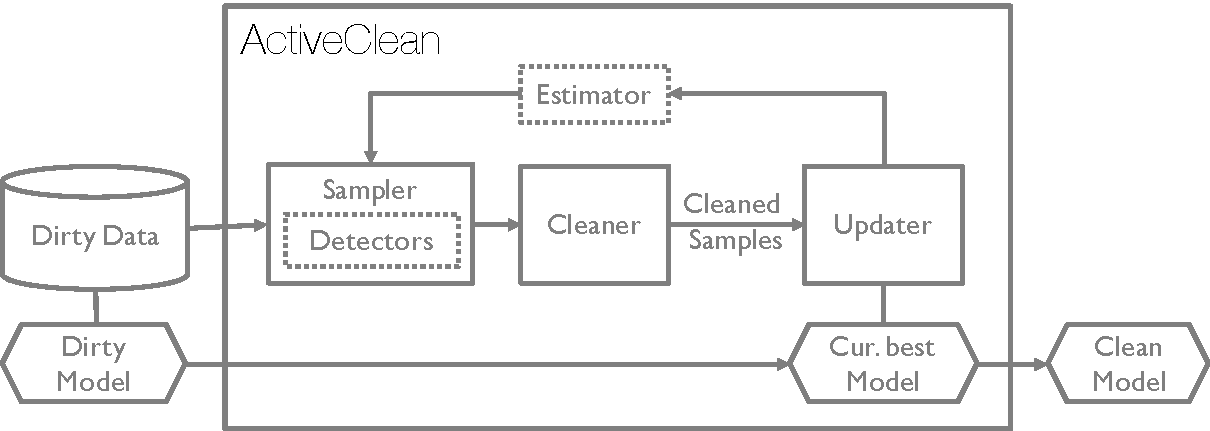
\includegraphics[width=\columnwidth]{figs/arch.pdf}
 \caption{\sysfull (\sys) is an anytime framework from training models on dirty data. Expensive data transformations prior to model training are budgeted with a non-uniform sampling that priortizes examples that are most likely to change the model. As more data is cleaned the sampling distribution is updated.  \label{sys-arch}}
\end{figure}

\subsection{Parameter Updates}
To achieve this architecture, \sys needs to maintain two states the parameter vector $\theta$ and the sampling distribution $P$.
We will formally describe the mathematics behind this process in the later sections.
In Figure \ref{param-arch}, we illustrate the structure of the parameter updates.
At each iteration, we draw a batch of dirty data using the sampling distribution $P$.
We calculate the average gradient for this data, and combine this gradient with the average gradient of the cleaned data.
We then update the parameter $\theta$ which in turn updates the sampling distribution.

\begin{figure}[t]
\centering
 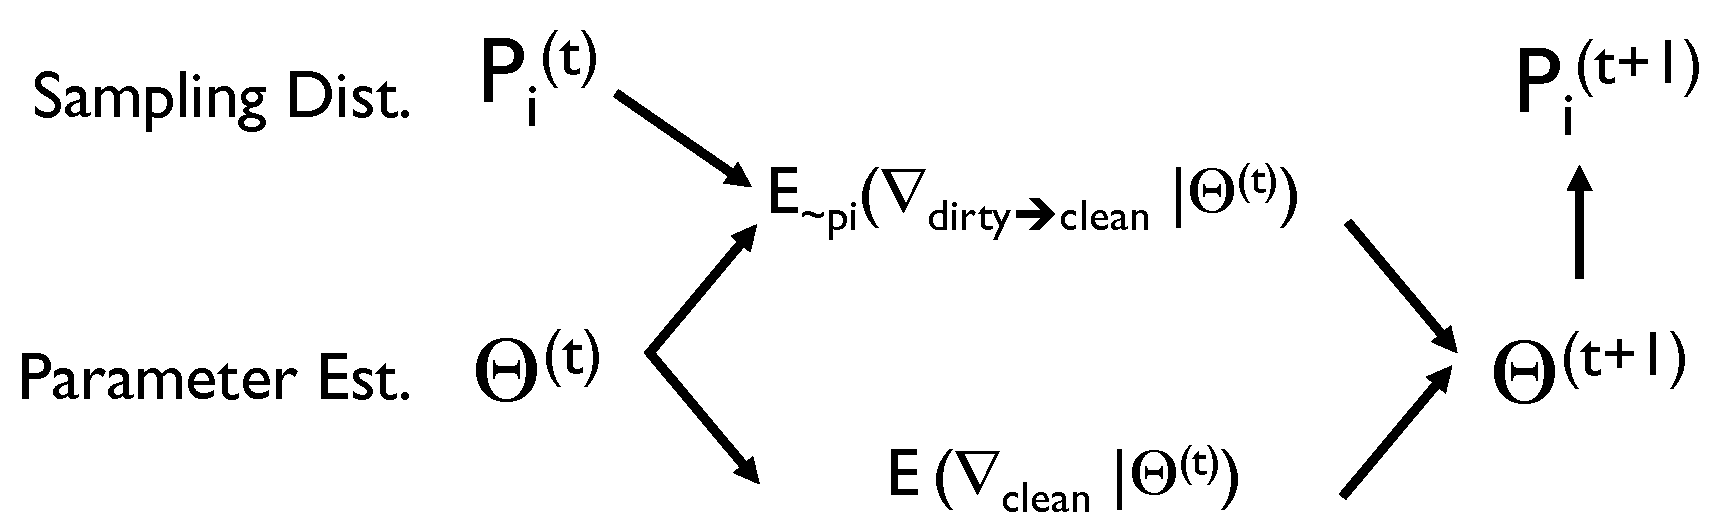
\includegraphics[width=\columnwidth]{figs/cmldag.pdf}
 \caption{The \sysfull operation DAG. At each iteration, we partition the data into clean and unknown quality. We fuse gradient estimates from the two partitions: (1) a sample from the unknown data using importance sampling, (2) a full (non-stochastic) gradient step on the clean data. After this estimate, we update the sampling distribution and the parameter.   \label{param-arch}}
\end{figure}


\iffalse
\subsection{Example Use Case And API}\label{api}
Consider the following example problem.
We are given the University of Texas Restaurant \footnote{http://www.cs.utexas.edu/users/ml/riddle/data/restaurant.tar.gz} dataset, which has the following schema:
\begin{lstlisting}[mathescape,basicstyle={\scriptsize}]
Restaurant(name$\textrm{,}$ address$\textrm{,}$ city$\textrm{,}$, type)
\end{lstlisting}
We want to train a Support Vector Machine classifier that given the tokens in the name and the city, can predict the category of the restaurant (e.g., Chinese or Mexican).
However, the challenge is that this dataset has numerous entity resolution problems where city names and categories are inconsistently represented.
\begin{lstlisting}[mathescape,basicstyle={\scriptsize}]
rex il ristorante,617 s. olive st.,los angeles,italian
rex il ristorante,617 s. olive st.,los angeles,nuova cucina italian
21 club,21 w. 52nd st.,new york,american
21 club,21 w. 52nd st.,new york city,american(new)
\end{lstlisting}
Entity resolution can be relatively expensive if the inconsistent representations are very different from each other and are not amenable to similarity measure optimizations such as prefix filtering or sorting.

\reminder{Maybe Describe API Here}

The analyst wants to quickly understand how much better a clean data set would be for this task.
Using our system, the analyst can construct a data cleaning workflow and specify a budget.
For example, this is what the code would look like in \sys.
\begin{lstlisting}[mathescape,basicstyle={\scriptsize}]
restaurant.load()

.clean(EntityResolution.weightedJaccard(`type',0.6))

.clean(EntityResolution.editDistance(`city',10))

.featureView(List(`type',`label'),(`city',`one_hot'),(`name',`bag_of_words')))

.model(new SVMModel(_))

.budget(5000)
\end{lstlisting}

\sys proposes an API for data cleaning pipeline construction. 
The API provides several data cleaning operations with known semantics.
Thus, we can use the lineage and operator semantics for optimization.
Of course, useful pipelines will often have User-Defined Functions and 
we will discuss the allowed operation types below.



\subsection{Algorithmic Problem Statement}
To formalize the optimization problem:

\noindent\textbf{Base Data and Featurization: } We are given a base dataset $\mathcal{R}$ which is a relation with $N$ rows. There is a featurization function $F$ which maps every row in $\mathcal{R}$ to a $d$ dimensional feature vector and a $l$ dimensional label tuple: \[F(r \in \mathcal{R}) \mapsto (\mathbb{R}^l, \mathbb{R}^d)\]. 

\noindent\textbf{Data Cleaning: } We define data cleaning as transformations that happens to the base data that result in changes to the feature vector. We do not consider data cleaning operations that change the number of rows in the relation such as row deletion or row deduplication. Allowed operations must result in the following changes to the feature vector: feature transformation and feature addition. Therefore, there is at most a one-to-one relationship beftween features in the cleaned data and the dirty data.

\reminder{Formalize Better}

\noindent\textbf{Budget Specification: } The analyst specifies two hyperparameters a cleaning budget $B$ which is the number of tuples to clean, and the number of cleaning rounds $T$. In each round, $\frac{B}{T}$ rows are processed by the system, we will discuss the tradeoffs between batching and incremental processing in the subsequent sections.

\reminder{Maybe exclude rounds}

\noindent\textbf{Model: } The analyst specifies the model which we require to be solved via convex regularized loss minimization:
\[
 \theta^{*}=\arg\min_{\theta}\sum_{i=1}^{N}\phi(x_{i},y_{i},\theta) + r(\theta)
\]

\noindent\textbf{Output: } The output of \sys is at each cleaning round we draw the sample of $\frac{B}{T}$ rows from a sampling distribution that incorporates information about the value of cleaning that row to model. After the $T$ cleaning rounds, the user is returned an approximately clean model $\theta^{(c)}$.
\fi
